%----------------------------------------------------------------------------
%----------------------------------------------------------------------------
%				    	SETUP
%----------------------------------------------------------------------------
%----------------------------------------------------------------------------

\documentclass[12pt]{article}

%----------------------------------------------------------------------------
%			  	   PACKAGES
%----------------------------------------------------------------------------

%% Fonts and Symbols
%% --------------------------
\usepackage[T1]{fontenc}			% better font encoding
\usepackage[utf8]{inputenc}		% better font encoding
%\usepackage[usenames,dvipsnames,svgnames,table]{xcolor}		% allow colour
\usepackage{amsmath,amssymb,amsthm,textcomp, xfrac}		% math symbols, etc
%\usepackage{color}
\usepackage[hidelinks]{hyperref}	% hyperlinks, see config in LAYOUT AND STYLING


%% Graphics
%% --------------------------
\usepackage{graphicx}			% allow insertion of images
\graphicspath{ {./graphics/} }		% the relative path to the graphics folder
\usepackage{subfigure}			% allows subfigures (a), (b), etc
%\usepackage{tikz}				% vector graphics
%\usepackage{pgfplots}			% plots in vector graphics


%% Tables
%% --------------------------
\usepackage{booktabs}			% better tables, discourages vertical rulings
%\usepackage{tabularx}
%\usepackage{enumerate}		
\usepackage{multicol}			%allow multi columns


%% Layout Alteration
%% --------------------------
\usepackage{lastpage}
\usepackage{fancyhdr}			% see config in LAYOUT AND STYLING
\usepackage{fullpage}			% set full page margins
%sideways figures
\usepackage{rotating}
%\usepackage{pdflscape}
\usepackage{parskip}			% disable indents
\usepackage{subfigure}			% allows for subfigures to have their own label

%% Units
%% --------------------------
\usepackage{siunitx}			% has S (decimal align) column type
\sisetup{input-symbols = {()},  % do not treat "(" and ")" in any special way
         group-digits  = false} % no grouping of digits
%\sisetup{load-configurations = abbreviations}
%\sisetup{per-mode = symbol}
%\usepackage{cancel}


%% Misc
%% --------------------------
%\usepackage{mhchem}			% chemistry


%----------------------------------------------------------------------------
%		     MACROS AND COMMANDS
%----------------------------------------------------------------------------

%type Y - even column width - centered
% must include tabularx package
%\newcolumntype{Y}{>{\centering\arraybackslash}X}	

% Defines a new command for the horizontal lines, change thickness here
\newcommand{\HRule}{\rule{\linewidth}{0.5mm}} 	

% ???
\newcommand{\linia}{\rule{\linewidth}{0.5pt}}

% scientific notation  use \e
\providecommand{\e}[1]{\ensuremath{\times 10^{#1}}}

% diferential
\def \d {\ensuremath{\mathrm{d}}}

%----------------------------------------------------------------------------
%		   	LAYOUT AND STYLING
%----------------------------------------------------------------------------

% custom footers and headers
% must include fancyhdr package
\pagestyle{fancy}
\lhead{}
\chead{}
\rhead{}
\lfoot{}
\cfoot{\thepage\ of \pageref{LastPage}}
\rfoot{}
\renewcommand{\headrulewidth}{0pt}
\renewcommand{\footrulewidth}{0pt}


%%section style
%\usepackage{titlesec}
%\titleformat{\section}[runin]
%{\normalfont\bfseries}
%{\thesection.}{.5em}{}[]
%
%\titleformat{\subsection}[runin]
%{\normalfont\bfseries}
%{\thesubsection}{.5em}{}[]
%\setcounter{secnumdepth}{0} %dont number sections

%\hypersetup{
%%    	colorlinks=false, 		% set true if you want colored links
%   		linktoc=all,     			% set to all if you want both sections and subsections linked
%%  		linkcolor=blue,  			% choose some color if you want links to stand out
%}


%----------------------------------------------------------------------------
%----------------------------------------------------------------------------
%				   DOCUMENT
%----------------------------------------------------------------------------
%----------------------------------------------------------------------------

\begin{document}

%----------------------------------------------------------------------------
%				    TITLE PAGE
%----------------------------------------------------------------------------

\begin{titlepage}

\center
 
% Header
\textsc{\LARGE University of Victoria}\\[1cm] 	% Name of your university/college
\textsc{\Large ELEC 250}\\[0.5cm] 			% Major heading such as course name
\textsc{\large Linear Circuits I}\\[0.5cm] 		% Minor heading such as course title


% Lab Title
\HRule \\[0.4cm]
{ \huge \bfseries Lab 3 - Transient Analysis}\\[0.2cm] % Title of your document
\HRule \\[1.5cm]
 
 
%Lab Instructor Details
\begin{minipage}{0.7\textwidth}
\begin{flushleft} 

\large\emph{Instructor:} \\
Dr. Nikitas \textsc{Dimopoulos} \\
\vspace{12 pt}
\emph{Teaching Assistant:} \\
Zhen \textsc{Liu}

\end{flushleft}
\end{minipage}
~
%% No content here, but it keeps the alignment of the instructor/TA
%% box correct.
%% Consider revising.
\begin{minipage}{0.1\textwidth}
\begin{flushright} \large
%Dr. Barbara \textsc{Sawicka} \\
\vspace{12 pt}
%\emph{Teaching Assistant:} \\
%Vahid \textsc{Moradi}
\end{flushright}
\end{minipage}\\[2cm]


% Lab members
\Large Clayton \textsc{Kihn}
\large V00794569	\\
\Large Yves \textsc{Senechal}
\large V00213837	\\
\Large Tyler \textsc{Stephen}
\large V00812021	\\
A01 - B01\\[1.5cm] 


% Date
{\large \today}\\ % Date, change the \today to a set date if you want to be precise

% Logo
\begin{figure}[b]	 % put logo at bottom of the page
	\centering
	\includegraphics[scale=0.3]{UVic_logo}
\end{figure}

\end{titlepage}

%----------------------------------------------------------------------------
%			  TABLE OF CONTENTS
%----------------------------------------------------------------------------

%\tableofcontents
%\pagebreak

%\listoffigures
%\pagebreak

%----------------------------------------------------------------------------
%				    BODY
%----------------------------------------------------------------------------

\section{Object}\label{sec:object}
This lab will study the transient response of an RC and an RL circuit.

\section{Results}\label{sec:results}
An Agilent 33220A signal generator was used to create the momentary single pulse excitation, while an Agilent DSOX-2012A oscilloscope was used to analyze transient responses of the RC and RL circuits. 


\subsection{RC Circuit}\label{sec:rc}
The circuit was constructed as shown in Figure \ref{fig:rc_circuit} and excited using a 5 V$_{pp}$ single pulse source for a duration of 5ms. 
\begin{figure}[h]
	\centering
	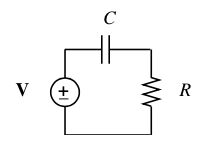
\includegraphics[scale = 0.75]{rc_circuit}
	\caption{RC circuit driven by a source. $R$ = 4.7 k$\Omega$ and $C$ = 100 nF. }
	\label{fig:rc_circuit}
\end{figure}

Measured values of the change in voltage across the capacitor and resistor in this circuit were recorded on the oscilloscope and are displayed in Figure \ref{fig:rc_meas}. In order to measure $v_R$, it was necessary to switch the order of $R$ and $C$.

The expected value of the time constant $\tau$ is given by
\begin{equation}\label{eqn:tau_rc}
	\tau = RC
\end{equation}

Using \eqref{eqn:tau_rc}, the expected value of $\tau$ is 480$\mu$s. By measuring the time it took for $v_C$ to decay to 37.25\% of its original value in Figure \ref{fig:rc_meas}.c, $\tau$ was determined to be 480$\mu$s.

\subsection{RL Circuit}\label{sec:rl}
The circuit was constructed as shown in Figure \ref{fig:rl_circuit} and excited using a 5 V$_{pp}$ single pulse source for a duration of 23.53$\mu$s.

\begin{figure}[h]
	\centering
	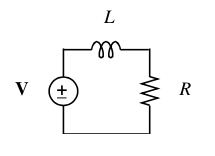
\includegraphics[scale = 0.75]{rl_circuit}
	\caption{RL circuit driven by a source. $R$ = 680 $\Omega$ and $L$ = 1.00 mH. }
	\label{fig:rl_circuit}
\end{figure}

Measured values of the change in voltage across the inductor and resistor in this circuit were recorded on the oscilloscope and are displayed in Figure \ref{fig:rl_meas}. In order to measure $v_R$, it was necessary to switch the order of $R$ and $L$.

The expected value of the time constant $\tau$ is given by
\begin{equation}\label{eqn:tau_rl}
	\tau = \frac{L}{R}
\end{equation}

Using \eqref{eqn:tau_rl}, the expected value of $\tau$ is 1.4$\mu$s. By measuring the time it took for $v_R$ to rise to 67.75\% of its final val in Figure \ref{fig:rl_meas}.c, $\tau$ was determined to be 1.4$\mu$s. The time for $v_L$ to decay to 37.25\% of its original value in Figure \ref{fig:rl_meas}.d yielded a $\tau$ of 1.34$\mu$s.

\section{Discussion and Conclusion}\label{sec:d_and_c}
The discussion and conclusion should answer the questions that are posed in the procedure section of the experiment. Any special observations made by the student can be recorded here.

\pagebreak
%% I can't find a way to fit the title and images on the same page... no matter how small the images are.
%\appendix
%\section{Scope Files}\label{app:scope}

\begin{sidewaysfigure}[h]
	\centering	
		\subfigure[$v_s$ and $v_R$]{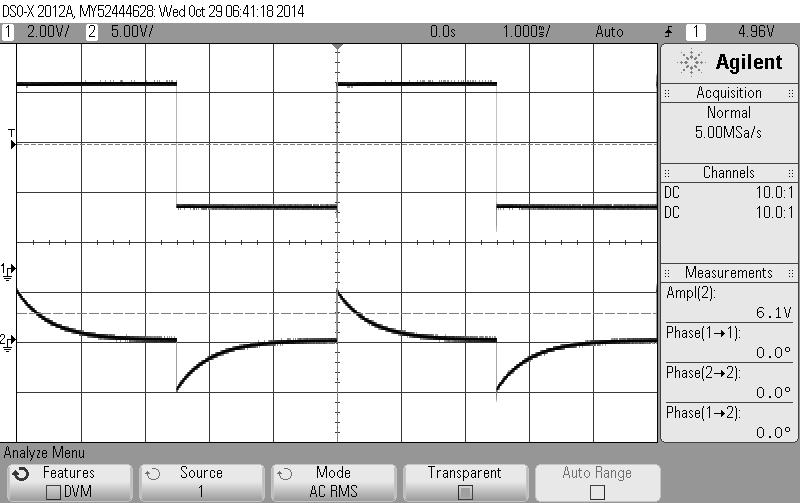
\includegraphics[width=0.475\textwidth]{scope_0}} \quad
		\subfigure[$v_s$ and $v_C$]{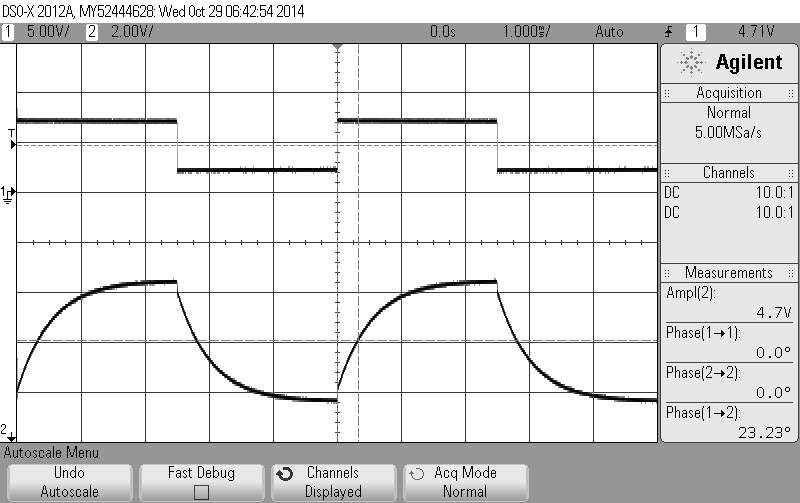
\includegraphics[width=0.475\textwidth]{scope_1}} \quad
		\subfigure[Decay of $v_C$ used to find $\tau$]{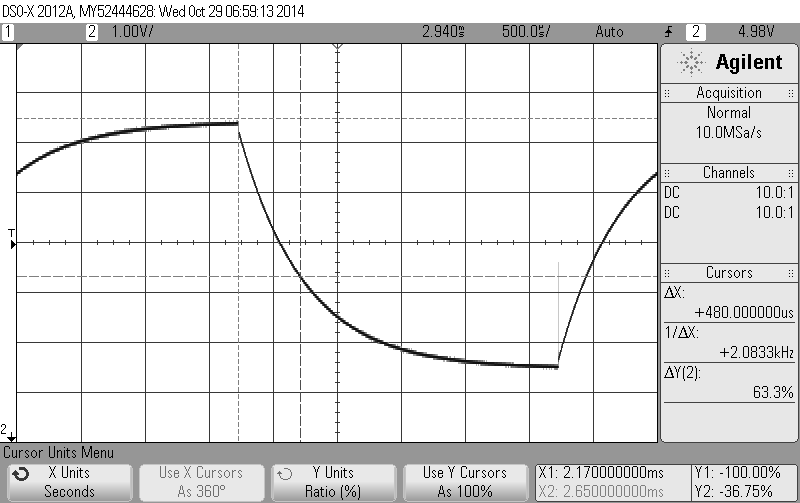
\includegraphics[width=0.475\textwidth]{scope_2}} 
	\caption{Transient response of the RC circuit}
	\label{fig:rc_meas}
\end{sidewaysfigure}

%\begin{sidewaysfigure}[h]
%	\centering	
%	\begin{subfigure}[b]{width=0.475\textwidth}
%		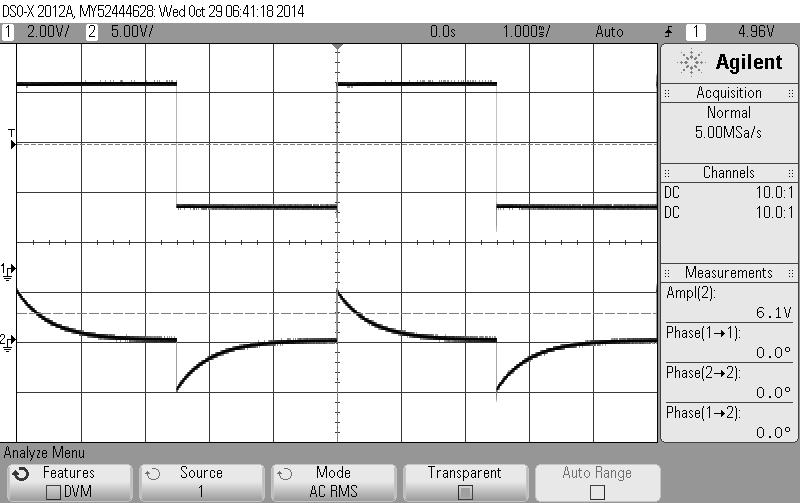
\includegraphics[width=\textwidth]{scope_0}
%		\caption{$v_s$ and $v_R$}
%		\label{sfig:1}	
%	\end{subfigure}%
%	\caption{Transient response of the RC circuit}
%	\label{fig:rc_meas}
%\end{sidewaysfigure}

\pagebreak

\begin{sidewaysfigure}[h]
	\centering	
		\subfigure[$v_s$ and $v_R$]{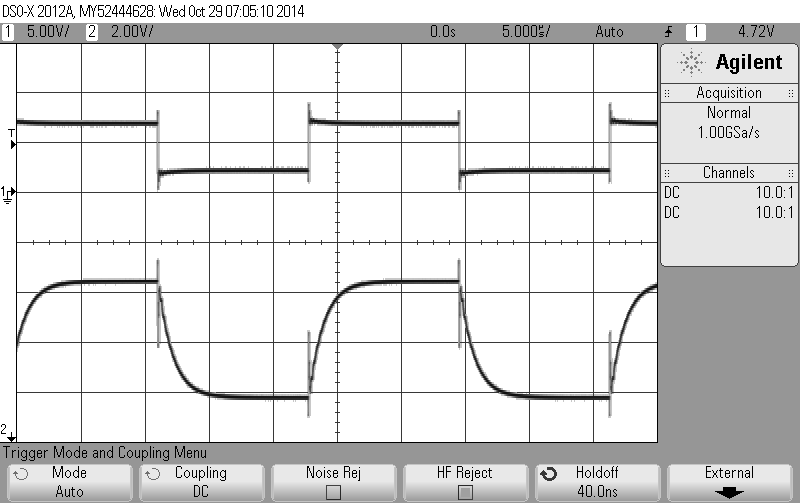
\includegraphics[width=0.475\textwidth]{scope_3}} \quad
		\subfigure[$v_s$ and $v_L$]{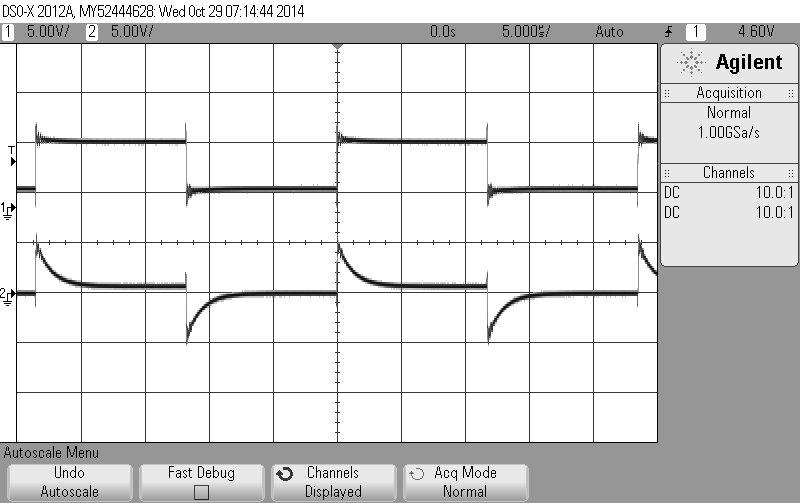
\includegraphics[width=0.475\textwidth]{scope_6}} \quad
		\subfigure[Rise of $v_R$ used to find $\tau$]{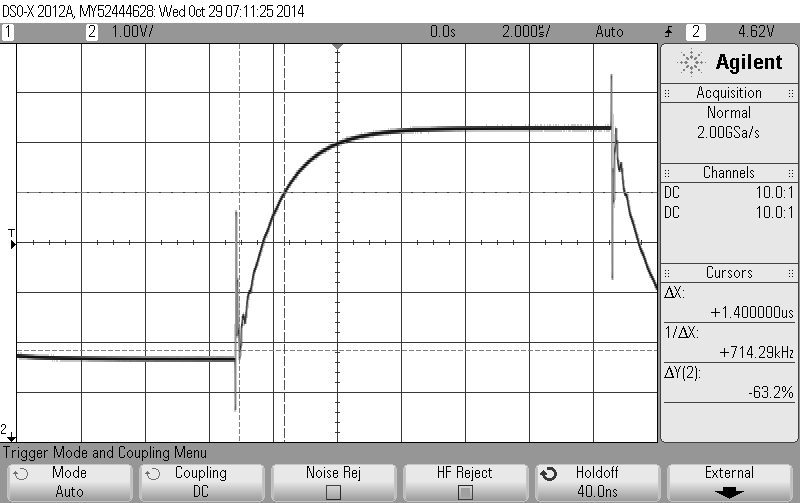
\includegraphics[width=0.475\textwidth]{scope_4}} \quad
		\subfigure[Decay of $v_L$ used to find $\tau$]{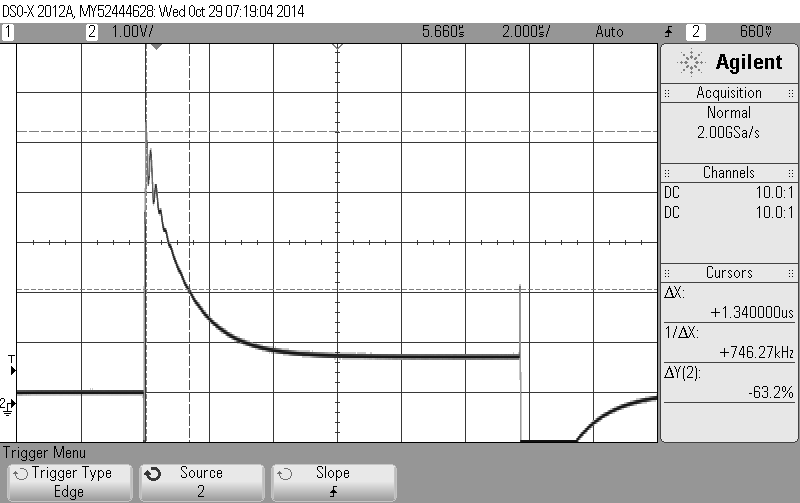
\includegraphics[width=0.475\textwidth]{scope_7}}
	\caption{Transient response of the RL circuit}
	\label{fig:rl_meas}
\end{sidewaysfigure}

%----------------------------------------------------------------------------
%				  LaTeX TIPS
%----------------------------------------------------------------------------

%\pagebreak
%
%\section{LaTeX Tips}\label{sec:tips}
%Check the source file for additional information in the comments.
%\subsection{Symbols}\label{sec:symbols}
%Most math symbols and all equations are bounded by \$ delimiters. \verb|$ A=\pi r^{2} $| produces $ A=\pi r^{2} $. To find the appropriate symbol you will have to use a LaTeX IDE with a built in symbol editor or use another program to produce the code and copy-and-paste it into your document.
%
%\subsection{Figures}\label{sec:figures}
%\begin{verbatim}
%\begin{figure}[h]
%	\centering
%	\includegraphics[width=0.75\textwidth]{Uvic_logo}
%	\caption{A logo used by the University of Victoria}
%	\label{fig:uvic_logo}
%\end{figure}
%\end{verbatim}
%
%\begin{figure}[h] 	% placement in document [htbp]: here, top, bottom, special page
%	\centering		% centers the image
%	\includegraphics[width=0.75\textwidth]{Uvic_logo} 	
%		% will search root directory and anything listed
%		% in \graphicspath for the image
%		% it is common to specify [width=0.5\textwidth] as an agument
%		% \textwidth can be used as a variable for the entire pagewidth.
%		% 0.5\textwidth refers to 50% of the page.
%	\caption{A logo used by the University of Victoria}
%	\label{fig:uvic_logo}
%\end{figure}
%
%A good tutorial for the use of figures can be found at: \url{http://en.wikibooks.org/wiki/LaTeX/Floats,_Figures_and_Captions}
%
%\pagebreak
%\subsection{Tables}\label{sec:tables}
%\begin{verbatim}
%\begin{table}[h]
%	\centering
%	\begin{tabular}{llr}
%		\hline
%		\multicolumn{2}{c}{Item} \\
%		\cline{1-2}
%			Animal   	& Description 	& Price (\$) \\
%		\hline
%			Gnat		& per gram	& 13.65      \\
%				        & each       	& 0.01       \\
%			Gnu		& stuffed     	& 92.50      \\
%			Emu		& stuffed		& 33.33      \\
%			Armadillo	& frozen		& 8.99       \\
%		\hline
%	\end{tabular}
%	\caption{Exotic meat prices}
%	\label{table:meats}
%\end{table}
%\end{verbatim}
%
%\begin{table}[h]			% placement in document [htbp]: [h]ere, [t]op, [b]ottom, special [p]age
%	\centering
%	\begin{tabular}{llr}	% specifies the number of columns and their justification
%					% columns can be [l]eft-justified, [c]entered, [r]ight-justified
%					% the number of arguments after {tabular} corresponds to the number of columns
%					% vertical lines can be added by placing | vertical bars in the argument
%					% e.g. { | c c c | } has three centered columns with vertical lines at the ends
%					% of the table
%					% { | c | c | c | } has vertical lines separating all cells
%
%		\hline		% a horizontal line
%		
%		\multicolumn{2}{c}{Item} \\		% {number of columns to span}{lcr}{title}
%								% \\ indicates the end of a line
%								
%		\cline{1-2}		% \cline[ i - j } : line that spans columns i to j
%		
%			Animal   	& Description 	& Price (\$) \\	% & separates data between cells
%											% && indicates a blank cell
%											% \\ must end every row
%		\hline
%			Gnat		& per gram	& 13.65      \\
%				        & each       	& 0.01       \\
%			Gnu		& stuffed     	& 92.50      \\
%			Emu		& stuffed		& 33.33      \\
%			Armadillo	& frozen		& 8.99       \\
%		\hline
%	\end{tabular}
%	\caption{Exotic meat prices}
%	\label{table:meats}
%\end{table}
%\textit{Apparently} tables are more readable if the vertical rulings are omitted. I'm inclined to agree.\\
%A good tutorial for the use of tables can be found at: \url{http://en.wikibooks.org/wiki/LaTeX/Tables}
%
%\subsection{Labels and References}\label{sec:labels_and_refs}
%LaTeX's dynamic referencing system gives it an advantage over other multi-user document tools. References point to assigned labels rather than a pre-defined numbering. Changing the order and number of references will leave the citations untouched if label referencing is used.
%
%
%The \verb|\label{}| tag should be attached to all sections, figures and tables. To reference these elements, use the \verb|\ref{}| command. To reference the table in Section \ref{sec:tables}, you would write \verb|Table \ref{table:meats}| which will appear as Table \ref{table:meats}.
%
%
%A consistent naming schema will make collaboration easier. Labels should be implemented with the corresponding prefix:
%\begin{table}[h]
%	\centering
%	\begin{tabular}{ l l }
%	Sections		& \verb|{sec:}|		\\
%	Figures		& \verb|{fig:}|		\\
%	Tables		& \verb|{table:}|		\\
%	\end{tabular}
%\end{table}
%
%You may encounter a situation where a citation or page number appears as \verb|??|. This often occurs when major changes have occured to the reference or page order. The LaTeX compiler requires two executions of the typesetting function to correctly address the references: one to build the .aux file and another to read from it. The compiler is often nice enouch to pass a warning when the .aux file has undergone significant changes to its references and prompts you do another typesetting.
%
%\subsection{Resources}\label{sec:resources}
%\begin{itemize}
%	\item \underline{\href{https://www.youtube.com/user/14mech14/videos}{Video playlist} } from McMaster that covers the installation and use of LaTeX. Uses TeXShop for examples. Covers document setup, tables, figures, bibliographies and some other stuff I haven't watched yet.
%\end{itemize}

%----------------------------------------------------------------------------
%----------------------------------------------------------------------------
%			DO NOT DELETE BELOW
%----------------------------------------------------------------------------
%----------------------------------------------------------------------------

\end{document}